\documentclass[11pt,a4paper]{article}

\usepackage[T1]{fontenc}
\usepackage[utf8]{inputenc}
\usepackage[margin=2.5cm]{geometry}
\usepackage{amsmath,amssymb,amsthm,mathtools}
\usepackage{booktabs,array,enumitem}
\usepackage{xcolor}
\usepackage[most]{tcolorbox}
\usepackage{tikz}
\usepackage{float}
\usetikzlibrary{arrows.meta,calc,positioning,decorations.markings,angles,quotes}
\usepackage{pgfplots}
\pgfplotsset{compat=1.17}
\usepackage{algpseudocode}
\usepackage[colorlinks=true,linkcolor=blue!50!black,urlcolor=blue!50!black]{hyperref}

% ---------- theorem-like environments ----------
\theoremstyle{definition}
\newtheorem{definition}{Definition}[section]
\newtheorem{example}[definition]{Example}
\theoremstyle{plain}
\newtheorem{theorem}[definition]{Theorem}
\newtheorem{proposition}[definition]{Proposition}
\newtheorem{lemma}[definition]{Lemma}
\theoremstyle{remark}
\newtheorem{remark}[definition]{Remark}

% ---------- Intuition box ----------
\newtcolorbox{intuition}{
  breakable, enhanced,
  colback=blue!6!white, colframe=blue!60!black,
  fonttitle=\bfseries, title=Intuition,
  left=5pt,right=5pt,top=3pt,bottom=3pt,
  before skip=10pt, after skip=10pt
}


% ---------- problem statement box ----------
\newtcolorbox{problem}[1]{
  breakable, enhanced,
  colback=black!4!white, colframe=black!65,
  fonttitle=\bfseries, title={#1},
  left=6pt,right=6pt,top=4pt,bottom=4pt,
  before skip=8pt, after skip=12pt
}

% ---------- algorithm box ----------
\newtcolorbox{algbox}[1]{
  breakable, enhanced,
  colback=gray!5!white, colframe=black!60,
  fonttitle=\bfseries, title={#1},
  left=5pt,right=5pt,
  before skip=10pt, after skip=10pt
}

% ---------- shortcuts ----------
\newcommand{\R}{\mathbb{R}}
\newcommand{\q}{\boldsymbol{q}}
\newcommand{\g}{\boldsymbol{g}}
\newcommand{\z}{\boldsymbol{z}}
\newcommand{\Tm}{\boldsymbol{T}}
\newcommand{\bb}{\boldsymbol{b}}
\newcommand{\dd}{\,\mathrm{d}}
\newcommand{\sgn}{\operatorname{sign}}
\newcommand{\rank}{\operatorname{rank}}
\newcommand{\SO}{\mathrm{SO}}

\title{\textbf{Autonomous and Mobile Robotics}\\[2pt]
\large Midterm Class Test Exercises: Hopping Robot, Chained Form Planning, Front-Wheel-Drive Bicycle}
\author{Lecture notes}
\date{}

\begin{document}
\maketitle
\tableofcontents
\bigskip

\noindent These notes work out in full three exercises on the kinematic modelling, controllability, flatness, planning and control of nonholonomic robots:
\begin{itemize}[nosep]
  \item the single-legged \textbf{hopping robot} in flight phase (Midterm 2022/23, Problem~1);
  \item \textbf{planning for a $(2,3)$ chained form} with a two-phase algorithm (Midterm 2021/22, Problem~2);
  \item the \textbf{front-wheel-drive bicycle}: kinematic model, controllability, (non-)flatness of the front wheel position and dynamic feedback linearization (Midterm 2024/25, Problem~1).
\end{itemize}
Each problem is solved part by part. Every non-obvious step is followed by a blue \emph{Intuition} box.

%=====================================================================
\section{Toolbox: the Recurring Ideas}
\label{sec:toolbox}
%=====================================================================

All three exercises are driftless nonholonomic systems, so the same few ideas keep returning. We collect them here.

\subsection{Pfaffian constraints and kinematic models}

A \emph{kinematic constraint} is linear in the generalized velocities,
\begin{equation}
  A^T(\q)\,\dot\q = 0, \qquad A(\q)\in\R^{n\times k},
\end{equation}
where $n=\dim\q$ and $k$ is the number of (independent) constraints. All admissible velocities lie in the $(n-k)$-dimensional null space of $A^T(\q)$. Choosing a basis $\g_1(\q),\dots,\g_{n-k}(\q)$ of this null space gives the \emph{kinematic model}
\begin{equation}
  \dot\q=\sum_{j=1}^{n-k}\g_j(\q)\,u_j = G(\q)\,u .
\end{equation}

\begin{intuition}
The constraint says ``you may not move in these $k$ directions'' (a wheel cannot skid sideways; angular momentum cannot be created from nothing). What is left is a space of allowed velocities, and the kinematic model simply parametrizes it with $n-k$ free numbers $u_j$.
The basis is \emph{not unique}: any invertible $u$-reparametrization gives an equivalent model. The good choice is the one in which the $u_j$ are quantities you can actually command, for instance joint velocities.
\end{intuition}

\subsection{Controllability by Lie brackets}

For driftless systems, controllability is decided by the \emph{accessibility rank condition}: if the involutive closure of $\operatorname{span}\{\g_1,\dots,\g_{n-k}\}$ (obtained by adding Lie brackets $[\g_i,\g_j]=\frac{\partial \g_j}{\partial \q}\g_i-\frac{\partial \g_i}{\partial \q}\g_j$, then brackets of brackets, \dots) has dimension $n$ at every $\q$, the system is controllable (Chow's theorem). If a constraint is \emph{nonholonomic} it is not integrable, so no loss of reachable configurations occurs: local velocity restrictions do not restrict global mobility.

\begin{intuition}
Think of parallel parking. You cannot slide the car sideways (a velocity restriction), yet you can reach any position by wiggling forward and backward while steering. The Lie bracket $[\g_i,\g_j]$ is the direction obtained by the sequence ``move along $\g_i$, then $\g_j$, then back along $\g_i$, then back along $\g_j$''; to first order the net displacement is along the bracket. Brackets are therefore the ``wiggle directions'' that are not available directly.
\end{intuition}

\subsection{Differential flatness and reconstruction}

A system $\dot\q=G(\q)u$ is \emph{differentially flat} with \emph{flat outputs} $y$ if $y$ has as many components as there are inputs, and $\q$ and $u$ can be reconstructed \emph{algebraically} (i.e.\ without integrating any differential equation) from $y$ and a finite number of its derivatives. For driftless systems, the \emph{geometric model} is obtained by replacing $\dot{(\cdot)}$ with $(\cdot)'=\mathrm d(\cdot)/\mathrm ds$ with respect to a path parameter $s$, and inputs $u$ by geometric inputs $\tilde u$ (so that $u=\tilde u\,\dot s$).
If $y$ is flat, a feasible path is planned by interpolating $y(s)$ with sufficiently smooth functions (e.g.\ polynomials) that match the boundary conditions, then reconstructing $\q(s)$ and $\tilde u(s)$.

\begin{intuition}
``Flat'' means the whole robot behaviour is encoded in a few free functions. Once you pick the curves $y(s)$ freely, nothing else is left to choose: the remaining states and inputs follow by differentiating and solving algebraic equations. This turns a planning problem with a nonholonomic constraint into a simple interpolation problem. The condition to check is whether the \emph{hidden} state variables can be recovered from $y$ without knowing an initial condition. If recovering a variable requires solving an ODE, it carries an arbitrary initial condition and $y$ is \emph{not} flat.
\end{intuition}

\subsection{Dynamic feedback linearization}

When the outputs to be controlled are such that the input does not appear in their first derivatives (or a static decoupling matrix is singular), one may \emph{extend the dynamics} by integrating some inputs. If after the extension the \emph{decoupling matrix} $\Tm$ in
\begin{equation}
  y^{(r)} = \bb(\q,\xi)+\Tm(\q,\xi)\,\tilde u
\end{equation}
is invertible, the choice $\tilde u=\Tm^{-1}(w-\bb)$ turns the system into $y^{(r)}=w$, i.e.\ decoupled chains of integrators, for which linear PD+feedforward tracking is available.

%=====================================================================
\section{The Single-Legged Hopping Robot}
\label{sec:hopper}
%=====================================================================
\emph{(Midterm Class Test 2022/23, Problem 1)}

\begin{problem}{Problem statement}
A simplified model of a single-legged hopping robot consists of a body with inertia moment $J$ and a leg of mass $m$. The leg is connected to the body through a revolute joint and a prismatic joint, which are separated by a distance $d$. Both joints are actuated; in particular, the extension of the length can be changed via the prismatic joint actuator.

When the robot is in flight phase, angular momentum is conserved. This leads to the following constraint
\[
  J\dot\theta+m(d+\ell)^2\dot\phi=0,
\]
where we have assumed that the leg mass is concentrated at its extremity (foot) and the initial momentum is zero.
Let the configuration of the robot be defined as $\q=(\phi,\ell,\theta)$ (the translational motion is not of interest).
\begin{enumerate}[label=(\alph*),nosep]
  \item Discuss the geometry of the robot configuration space.
  \item Derive a kinematic model of the robot for which there is a clear physical interpretation of the associated inputs.
  \item Discuss local and global mobility of the robot in its configuration space.
  \item Using the kinematic model, find a feedback control law for the flight phase that will drive the body orientation $\theta$ to zero and the leg length to a constant value $h$. Provide a block scheme.
  \item Consider for simplicity the case $d=0$. Show that the system is differentially flat and derive the associated reconstruction formulas. Based on this, devise an algorithm for planning a feasible path between two arbitrary configurations $\q_s$ and $\q_g$.
\end{enumerate}
\end{problem}


\subsection{Setting}

A simplified single-legged hopping robot consists of a body with inertia moment $J$ and a leg of mass $m$ concentrated at its extremity (the foot). The leg is attached to the body through a revolute joint and a prismatic joint, separated by a distance $d$; both are actuated, so the leg length $\ell$ can be changed. Let $\phi$ be the leg angle (relative to the horizontal), $\ell$ the leg extension and $\theta$ the body orientation. Only the orientation-related motion is of interest, so
\[
  \q=(\phi,\ell,\theta)^T .
\]

\begin{figure}[H]
\centering
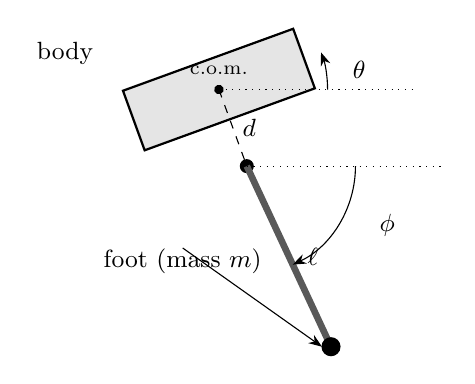
\begin{tikzpicture}[scale=1.15, >=Stealth]
  % reference
  \coordinate (B) at (0,0);
  % body rotated by theta=20 deg
  \begin{scope}[rotate=20]
    \draw[thick,fill=gray!20] (-1.0,-0.35) rectangle (1.0,0.35);
    \fill (0,0) circle (1.5pt) node[above=2pt,font=\scriptsize] {c.o.m.};
  \end{scope}
  % revolute joint at distance d below body center along body-normal
  \coordinate (P) at ($(B)+(20-90:0.9)$);
  \draw[dashed] (B) -- (P) node[midway,right,font=\small]{$d$};
  \fill (P) circle (2.2pt);
  % leg: angle phi=-65 deg from horizontal
  \coordinate (Fo) at ($(P)+(-65:2.2)$);
  \draw[line width=2.4pt,gray!70!black] (P) -- (Fo);
  \fill (Fo) circle (3pt);
  \node[right,font=\small] at ($(P)!0.5!(Fo)+(0.1,0)$) {$\ell$};
  % reference horizontals
  \draw[dotted] (B) -- ++(2.2,0);
  \draw[dotted] (P) -- ++(2.2,0);
  % theta arc
  \draw[->] (1.2,0) arc[start angle=0,end angle=20,radius=1.2];
  \node[font=\small] at (1.55,0.22) {$\theta$};
  % phi arc
  \draw[->] ($(P)+(1.2,0)$) arc[start angle=0,end angle=-65,radius=1.2];
  \node[font=\small] at ($(P)+(1.55,-0.65)$) {$\phi$};
  \node[font=\small] at (-1.7,0.4) {body};
  \node[font=\small] at (-0.4,-1.9) {foot (mass $m$)};
  \draw[->,thin] (-0.4,-1.75) -- ($(Fo)+(-0.1,0.0)$);
\end{tikzpicture}
\caption{Schematic of the hopping robot: body with inertia $J$ and orientation $\theta$, revolute joint (angle $\phi$) and prismatic joint (extension $\ell$) separated by $d$. Original redrawing.}
\end{figure}

During the flight phase the total angular momentum is conserved. With zero initial momentum and the leg mass concentrated at the foot,
\begin{equation}
  J\dot\theta+m(d+\ell)^2\dot\phi=0 .
  \label{eq:hop-constraint}
\end{equation}

\begin{intuition}
This is the same principle that lets a falling cat turn in mid-air, or an astronaut reorient without touching anything: with no external torque, total angular momentum stays zero, so rotating the leg one way forces the body to rotate the other way. How \emph{much} the body turns depends on the lever arm $(d+\ell)$ of the leg: since $\dot\theta=-\frac{m(d+\ell)^2}{J}\dot\phi$, a \emph{longer} leg produces \emph{more} body rotation for the same swing. This lever-arm effect is what makes the robot controllable in part~(c).
\end{intuition}

\subsection{(a) Geometry of the configuration space}

Both $\phi$ and $\theta$ are angles, hence elements of $\SO(2)$ (circles), whereas the extension $\ell$ is a real number (physically $\ell\ge0$). Therefore
\[
  \mathcal C=\SO(2)\times\R\times\SO(2),\qquad n=\dim\mathcal C=3 .
\]
There is a single constraint, \eqref{eq:hop-constraint}, so $k=1$.

\begin{intuition}
The configuration space is not $\R^3$ but a ``cylinder times a circle'': angles wrap around ($\phi$ and $\phi+2\pi$ are the same configuration). This matters later, when planning: reaching $\phi_g$ may be done by choosing any representative $\phi_g+2\pi k$, which changes the path.
\end{intuition}

\subsection{(b) A kinematic model with physically meaningful inputs}

Writing \eqref{eq:hop-constraint} in Pfaffian form,
\begin{equation}
  \underbrace{\begin{pmatrix} m(d+\ell)^2 & 0 & J\end{pmatrix}}_{A^T(\q)}
  \begin{pmatrix}\dot\phi\\ \dot\ell\\ \dot\theta\end{pmatrix}=0 .
\end{equation}
The null space of $A^T(\q)$ has dimension $n-k=2$. Two vector fields spanning it are
\begin{equation}
  \g_1(\q)=\begin{pmatrix}1\\0\\ -\frac{m(d+\ell)^2}{J}\end{pmatrix},\qquad
  \g_2(\q)=\begin{pmatrix}0\\1\\0\end{pmatrix},
\end{equation}
which gives the kinematic model
\begin{equation}
\boxed{\;
\begin{aligned}
  \dot\phi&=u_1\\
  \dot\ell&=u_2\\
  \dot\theta&=-\frac{m(d+\ell)^2}{J}\,u_1 .
\end{aligned}\;}
\label{eq:hop-km}
\end{equation}

\emph{How the basis is found.} We want $\dot\phi$ and $\dot\ell$ to be the inputs, since they are the velocities of the two actuated joints. Hence the first two components of the basis vectors should be $(1,0)$ and $(0,1)$. The third component $\alpha$ of $\g_1=(1,0,\alpha)^T$ is fixed by requiring $A^T\g_1=0$:
\[
  m(d+\ell)^2+J\alpha=0\;\Longrightarrow\;\alpha=-\frac{m(d+\ell)^2}{J},
\]
while $\g_2=(0,1,0)^T$ is automatically in the null space since the constraint does not involve $\dot\ell$.

\begin{intuition}
The model says: command the two joints freely ($u_1$ swings the leg, $u_2$ extends it), and the body orientation is \emph{slaved} to the leg swing through the conservation of angular momentum. $\dot\ell=u_2$ does not affect $\theta$ at all, as extending the leg exerts no torque about the center of mass in this model, but \emph{when} you swing depends on $\ell$. Any other basis is equally valid mathematically (e.g.\ taking $\dot\theta$ as an input), but then the inputs would no longer be joint velocities.
\end{intuition}

\subsection{(c) Local and global mobility}

\paragraph{Local mobility.} At each $\q$, the velocity $\dot\q$ must belong to $\mathcal N(A^T(\q))$, a 2-dimensional subspace of the 3-dimensional tangent space. So \emph{locally} the robot cannot move in an arbitrary direction: the body cannot rotate independently of the leg.

\paragraph{Global mobility.} We check the accessibility rank condition. The only non-trivial bracket is
\begin{equation}
  \g_3(\q)=[\g_1,\g_2](\q)=\frac{\partial\g_2}{\partial\q}\g_1-\frac{\partial\g_1}{\partial\q}\g_2
  =-\frac{\partial\g_1}{\partial\ell}
  =\begin{pmatrix}0\\0\\ \dfrac{2m(d+\ell)}{J}\end{pmatrix}.
\end{equation}
Its third component never vanishes provided $d+\ell>0$ (this holds for $\ell\ge0$ as soon as $d>0$; if $d=0$ the point $\ell=0$ is singular, where the leg has no lever arm). Hence
\[
  \rank\begin{pmatrix}\g_1&\g_2&\g_3\end{pmatrix}=3 ,
\]
and the kinematic model is \emph{controllable}. In other words, the angular-momentum conservation constraint is \emph{nonholonomic}: global mobility is not restricted, and every configuration of $\mathcal C$ can be reached.

\begin{intuition}
Here is the concrete ``wiggle'' behind the bracket. Take $m/J=1$, $d=0$. Extend the leg to $\ell_2=2$, swing it by $\Delta\phi=0.5$\,rad, retract to $\ell_1=1$, and swing back by $-0.5$\,rad. The body rotation produced while swinging out is $-\ell_2^2\Delta\phi=-2$\,rad; the one while swinging back is $+\ell_1^2\Delta\phi=+0.5$\,rad. The leg is back at the same $(\phi,\ell)$, but the body has rotated by
\[
  \Delta\theta=-\frac{m}{J}\Delta\phi\,\big[(d+\ell_2)^2-(d+\ell_1)^2\big]=-0.5\,(4-1)=-1.5\ \text{rad}.
\]
So a closed cycle in the leg variables $(\phi,\ell)$ produces a net rotation of the body: this is why one can reorient arbitrarily in flight (exactly like the cat), and it is the geometric meaning of $\g_3$ pointing along $\theta$.
\end{intuition}

\begin{figure}[H]
\centering
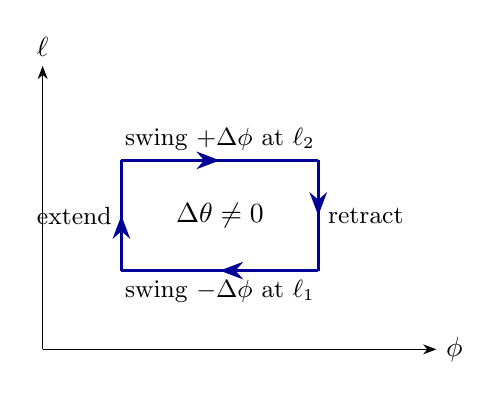
\begin{tikzpicture}[>=Stealth,scale=1.0]
  \draw[->] (0,0) -- (5,0) node[right]{$\phi$};
  \draw[->] (0,0) -- (0,3.6) node[above]{$\ell$};
  \draw[very thick,blue!60!black,
        decoration={markings,mark=at position 0.5 with {\arrow{Stealth}}},postaction={decorate}]
        (1,1) -- (1,2.4) ;
  \draw[very thick,blue!60!black,
        decoration={markings,mark=at position 0.5 with {\arrow{Stealth}}},postaction={decorate}]
        (1,2.4) -- (3.5,2.4);
  \draw[very thick,blue!60!black,
        decoration={markings,mark=at position 0.5 with {\arrow{Stealth}}},postaction={decorate}]
        (3.5,2.4) -- (3.5,1);
  \draw[very thick,blue!60!black,
        decoration={markings,mark=at position 0.5 with {\arrow{Stealth}}},postaction={decorate}]
        (3.5,1) -- (1,1);
  \node[left,font=\small] at (1,1.7) {extend};
  \node[above,font=\small] at (2.25,2.4) {swing $+\Delta\phi$ at $\ell_2$};
  \node[right,font=\small] at (3.5,1.7) {retract};
  \node[below,font=\small] at (2.25,1) {swing $-\Delta\phi$ at $\ell_1$};
  \node at (2.25,1.7) {$\Delta\theta\ne0$};
\end{tikzpicture}
\caption{A rectangular loop in the leg variables $(\phi,\ell)$ leaves the leg where it started but produces a net body rotation $\Delta\theta$ (nonholonomy).}
\end{figure}

\subsection{(d) Feedback control in flight: $\theta\to0$, $\ell\to h$}

In the model \eqref{eq:hop-km} the leg length is a pure integrator, $\dot\ell=u_2$. Choosing
\begin{equation}
  u_2=k_\ell\,(h-d-\ell),\qquad k_\ell>0,
  \label{eq:hop-u2}
\end{equation}
gives $\dot\ell=-k_\ell(\ell-(h-d))$, i.e.\ exponential convergence of $\ell$ to $h-d$, so that the total leg length $d+\ell$ converges to the desired $h$.

For $\theta$, introduce the input transformation (always invertible, since $d+\ell>0$)
\[
  u_1=-\frac{J}{m(d+\ell)^2}\,v_1 ,
\]
under which $\dot\theta=v_1$. Taking $v_1=-k_\theta\theta$, $k_\theta>0$, yields exponential convergence of $\theta$ to zero. Going back to the original input:
\begin{equation}
  u_1=k_\theta\,\frac{J}{m(d+\ell)^2}\,\theta .
  \label{eq:hop-u1}
\end{equation}
The control law \eqref{eq:hop-u2}--\eqref{eq:hop-u1} only needs measurements of $\ell$ and $\theta$ (not $\phi$).

\begin{figure}[H]
\centering
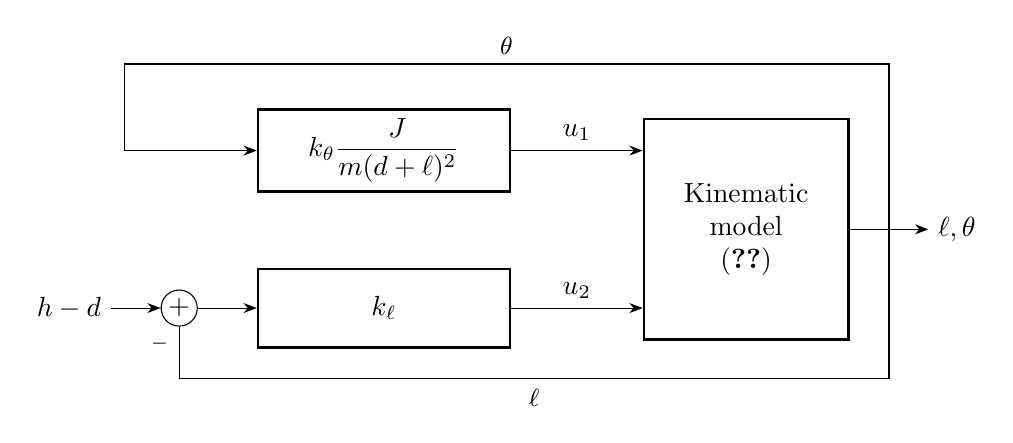
\begin{tikzpicture}[>=Stealth,
  blk/.style={draw,thick,rectangle,minimum height=1.0cm,minimum width=3.2cm,align=center}]
  \node[blk] (c1) at (0,1.6) {$k_\theta\dfrac{J}{m(d+\ell)^2}$};
  \node[blk] (c2) at (0,-0.4) {$k_\ell$};
  \node[circle,draw,inner sep=1pt] (sum) at (-2.6,-0.4) {$+$};
  \node (h) at (-4.0,-0.4) {$h-d$};
  \node[blk,minimum height=2.8cm,minimum width=2.6cm] (plant) at (4.6,0.6) {Kinematic\\model\\\eqref{eq:hop-km}};
  \draw[->] (h) -- (sum);
  \draw[->] (sum) -- (c2);
  \draw[->] (c1.east) -- node[above]{$u_1$} (c1.east -| plant.west);
  \draw[->] (c2.east) -- node[above]{$u_2$} (c2.east -| plant.west);
  \draw[->] (plant.east) -- ++(1.0,0) node[right]{$\ell,\theta$};
  % theta feedback
  \draw[->] ($(plant.east)+(0.5,0)$) -- ++(0,2.1) -| node[pos=0.25,above,font=\small]{$\theta$} (-3.3,1.6) -- (c1.west);
  % l feedback
  \draw ($(plant.east)+(0.5,0)$) -- ++(0,-1.9) -| node[pos=0.25,below,font=\small]{$\ell$} (sum.south);
  \node[font=\scriptsize] at (-2.85,-0.85) {$-$};
\end{tikzpicture}
\caption{Block scheme of the flight-phase controller: two decoupled loops. The $\theta$-loop applies the state-dependent gain $k_\theta J/(m(d+\ell)^2)$ to $\theta$ (regulation to zero); the $\ell$-loop is a proportional regulator on $h-d-\ell$.}
\end{figure}

\begin{intuition}
The trick is to make each variable look like a trivial first-order system $\dot x=-kx$. For $\ell$ this is immediate. For $\theta$, the factor $\frac{m(d+\ell)^2}{J}$ is a (known, positive) ``gear ratio'' between the swing velocity $u_1$ and the body rotation rate, so we simply divide by it. The price is that $\phi$ is left uncontrolled: it drifts. How far? If $\ell$ were constant, momentum conservation gives $J\Delta\theta=-m(d+\ell)^2\Delta\phi$. Straightening the body from $\theta_0=0.3$\,rad with $d+\ell=h=0.5$\,m, $m/J=2\,\mathrm{m^{-2}}$ requires the leg to rotate by
\[
  \Delta\phi=\frac{J}{m h^2}\theta_0=\frac{0.3}{2\cdot0.25}=0.6\ \text{rad}.
\]
\end{intuition}

\subsection{(e) Differential flatness for $d=0$ and path planning}

For $d=0$ the model \eqref{eq:hop-km} becomes
\begin{equation}
\begin{aligned}
  \dot\phi&=u_1\\ \dot\ell&=u_2\\ \dot\theta&=-\frac{m\ell^2}{J}u_1 .
\end{aligned}
\label{eq:hop-d0}
\end{equation}

\begin{proposition}
System \eqref{eq:hop-d0} is differentially flat with flat outputs $(\phi,\theta)$.
\end{proposition}

\begin{proof}
Using $u_1=\dot\phi$ in the last equation gives $\ell^2=-\frac{J}{m}\frac{\dot\theta}{\dot\phi}$. Since $\ell\ge0$,
\begin{equation}
  \ell=\sqrt{-\frac{J}{m}\frac{\dot\theta}{\dot\phi}} .
  \label{eq:hop-ell}
\end{equation}
The inputs follow immediately:
\begin{equation}
  u_1=\dot\phi,\qquad
  u_2=\dot\ell=\frac{1}{2\ell}\left(-\frac{J}{m}\right)\frac{\ddot\theta\dot\phi-\dot\theta\ddot\phi}{\dot\phi^2}
  =\frac{J}{2m\ell}\,\frac{\dot\theta\ddot\phi-\ddot\theta\dot\phi}{\dot\phi^2},
  \label{eq:hop-u2rec}
\end{equation}
with $\ell$ given by \eqref{eq:hop-ell}. All reconstruction formulas are algebraic in $(\phi,\theta)$ and their derivatives (up to second order), so $(\phi,\theta)$ is a flat output.
\end{proof}

\begin{remark}
Constraint \eqref{eq:hop-constraint} implies that $\dot\theta$ and $\dot\phi$ always have \emph{opposite} signs, so the radicand in \eqref{eq:hop-ell} is nonnegative: the square root is well-posed, and $\ell>0$ is consistent with the constraint. The formulas require $\dot\phi\neq0$.
\end{remark}

\begin{intuition}
Why is $\ell$ \emph{not} a flat output while $\theta$ is? Because $\ell$ can be read off from the \emph{ratio} of how fast the body turns to how fast the leg swings: a long leg turns the body a lot per unit swing. So watching $\phi(t)$ and $\theta(t)$ is enough to infer the leg length at every instant, and then its rate, and the input.
\end{intuition}

\paragraph{Planning.} For path planning we use the geometric version of \eqref{eq:hop-d0}, where $(\cdot)'=\mathrm d/\mathrm ds$:
\begin{equation}
  \phi'=\tilde u_1,\qquad \ell'=\tilde u_2,\qquad \theta'=-\frac{m\ell^2}{J}\tilde u_1 .
  \label{eq:hop-geo}
\end{equation}
Time has disappeared: only the \emph{shape} of the path matters. The reconstruction formulas hold with $s$-derivatives:
\[
  \ell=\sqrt{-\tfrac{J}{m}\tfrac{\theta'}{\phi'}},\qquad
  \tilde u_1=\phi',\qquad
  \tilde u_2=\ell'=\frac{J}{2m\ell}\,\frac{\theta'\phi''-\theta''\phi'}{\phi'^2}.
\]

\begin{algbox}{Algorithm: path planning between $\q_s=(\phi_s,\ell_s,\theta_s)$ and $\q_g=(\phi_g,\ell_g,\theta_g)$ ($d=0$)}
\begin{algorithmic}[1]
  \State Choose a \textbf{linear} polynomial $\phi(s)=as+b$, $s\in[0,1]$, with $\phi(0)=\phi_s$, $\phi(1)=\phi_g$.
  \Statex \hspace{\algorithmicindent} Hence $b=\phi_s$, $a=\phi_g-\phi_s$, and $\tilde u_1(s)=\phi'(s)=a$ for all $s$.
  \State Choose a \textbf{cubic} polynomial $\theta(s)=cs^3+ds^2+es+f$ with
  \Statex \hspace{\algorithmicindent} $\theta(0)=\theta_s$, $\theta(1)=\theta_g$,
  \Statex \hspace{\algorithmicindent} $\theta'(0)=-\dfrac{m\,\ell_s^2}{J}\,a$, $\quad\theta'(1)=-\dfrac{m\,\ell_g^2}{J}\,a$.
  \State Reconstruct $\ell(s)=\sqrt{-\frac{J}{m}\frac{\theta'(s)}{a}}$ and $\tilde u_2(s)=\ell'(s)$.
  \State (Optional) Pick a time law $s(t)$ to obtain velocities $u=\tilde u\,\dot s$.
\end{algorithmic}
\end{algbox}

The boundary conditions on $\theta'$ come from the last equation of \eqref{eq:hop-geo} with $\tilde u_1=a$: they \emph{encode the initial and final leg lengths}. Solving the four linear conditions on the cubic, with $\Delta\theta=\theta_g-\theta_s$ and $\theta'_s,\theta'_g$ the two prescribed slopes,
\[
  f=\theta_s,\quad e=\theta'_s,\quad d=3\Delta\theta-2\theta'_s-\theta'_g,\quad c=\theta'_s+\theta'_g-2\Delta\theta .
\]

\begin{intuition}
Why a line for $\phi$ and a cubic for $\theta$? $\phi$ only has two boundary conditions (start and end value), so a straight line suffices, and conveniently gives a \emph{constant} geometric input $a$. $\theta$ has four conditions (two values and two slopes), so we need a cubic. The two slope conditions are what carry the information about $\ell_s$ and $\ell_g$: they say ``the body must be turning, at the start, at the rate corresponding to leg length $\ell_s$, and at the end at the rate corresponding to $\ell_g$''. Once $\theta(s)$ is fixed, the leg length in between is whatever is needed to make the constraint hold.
\end{intuition}

\begin{remark}[Feasibility check]
Since $\ell^2=-\frac{J}{m}\frac{\theta'}{a}$ must be positive along the whole path, the cubic must satisfy $a\,\theta'(s)<0$ for all $s\in[0,1]$: its derivative must not change sign. The boundary slopes already have the right sign; if the interior of $\theta'$ crosses zero, the plan is not feasible and one must modify it (e.g.\ choose $\phi_g+2\pi k$, i.e.\ a different number of leg turns, or use a higher-degree polynomial). If $\phi_s=\phi_g$ then $a=0$ and the formulas degenerate (a nonconstant $\phi(s)$ must be chosen).
\end{remark}

\begin{example}[Numerical example]
Take $m/J=1$, $\phi:0\to1$ (so $a=1$), $\ell_s=1$, $\ell_g=1.5$, and $\theta_s=0$, $\theta_g=-2$. Then $\theta'_s=-1$, $\theta'_g=-2.25$, $\Delta\theta=-2$, so
\[
  c=-1-2.25+4=0.75,\quad d=-6+2+2.25=-1.75,\quad e=-1,\quad f=0,
\]
\[
  \theta(s)=0.75s^3-1.75s^2-s,\qquad
  \ell(s)=\sqrt{-\theta'(s)}=\sqrt{1+3.5s-2.25s^2}.
\]
Here $\theta'(s)=2.25s^2-3.5s-1$ has its roots at $s\approx-0.25$ and $s\approx1.8$, outside $[0,1]$, so $\theta'<0$ throughout and the path is feasible; indeed $\ell(0)=1$ and $\ell(1)=1.5$.
\end{example}

\begin{figure}[H]
\centering
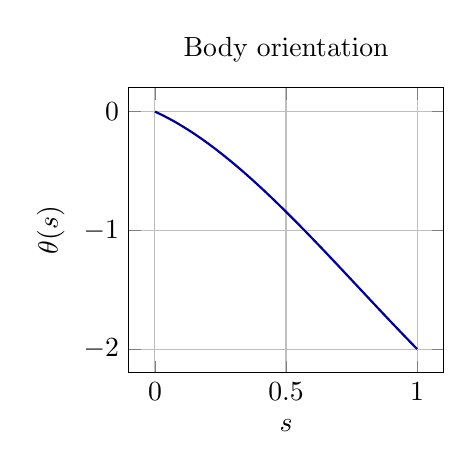
\begin{tikzpicture}
\begin{axis}[width=0.46\textwidth,height=5.2cm,xlabel={$s$},ylabel={$\theta(s)$},grid=both,
  domain=0:1,samples=60,title={Body orientation}]
  \addplot[thick,blue!60!black]{0.75*x^3-1.75*x^2-x};
\end{axis}
\end{tikzpicture}\hfill
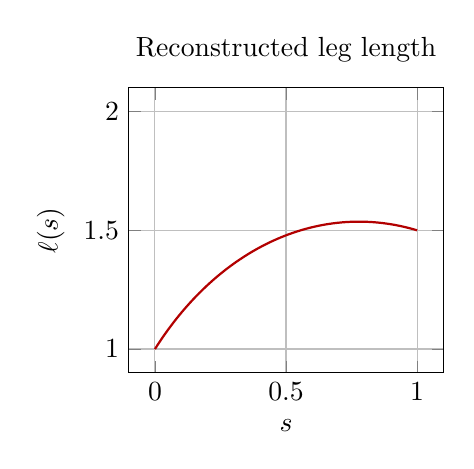
\begin{tikzpicture}
\begin{axis}[width=0.46\textwidth,height=5.2cm,xlabel={$s$},ylabel={$\ell(s)$},grid=both,
  domain=0:1,samples=60,title={Reconstructed leg length},ymin=0.9,ymax=2.1]
  \addplot[thick,red!70!black]{sqrt(1+3.5*x-2.25*x^2)};
\end{axis}
\end{tikzpicture}
\caption{Planned path for the numerical example: the cubic $\theta(s)$ and the leg length $\ell(s)$ reconstructed from it. Note how $\ell(s)$ is never freely chosen: it is imposed by $\theta$.}
\end{figure}

%=====================================================================
\section{Planning for a $(2,3)$ Chained Form}
\label{sec:chained}
%=====================================================================
\emph{(Midterm Class Test 2021/22, Problem~2)}

\begin{problem}{Problem statement}
Consider a $(2,3)$ chained form. It is easy to verify that the application of the control inputs
\[
  v_1=a\sin\omega t,\qquad v_2=b\cos\omega t
\]
over the time interval $[0,2\pi/\omega]$ brings $z_1,z_2$ back to their initial values and causes a displacement of $z_3$ equal to $ab\pi/\omega^2$. Exploiting this fact (no need to prove it), design a 2-phase algorithm for planning a trajectory that moves the chained form system from any initial configuration $\z_i$ to any final configuration $\z_f$. Moreover:
\begin{enumerate}[label=(\alph*),nosep]
  \item provide a pseudocode description of the algorithm;
  \item discuss which are its free parameters and how to choose their values;
  \item assuming $\z_i=(0,0,0)$ and $\z_f=(1,1,1)$, compute the total time needed for reaching $\z_f$ and draw the trajectory of the system on the $z_1,z_2$ plane.
\end{enumerate}
\end{problem}


\subsection{Setting}

The $(2,3)$ chained form has two inputs and three states:
\begin{equation}
  \dot z_1=v_1,\qquad \dot z_2=v_2,\qquad \dot z_3=z_2\,v_1 .
  \label{eq:chain}
\end{equation}
We are given the fact that the sinusoidal inputs
\[
  v_1=a\sin\omega t,\qquad v_2=b\cos\omega t
\]
applied over $[0,2\pi/\omega]$ bring $z_1,z_2$ back to their initial values and produce a displacement $\Delta z_3=ab\pi/\omega^2$. We exploit it to design a two-phase algorithm moving $\z_i=(z_{1,i},z_{2,i},z_{3,i})$ to any $\z_f=(z_{1,f},z_{2,f},z_{3,f})$.

\paragraph{Controllability check.} With $\g_1=(1,0,z_2)^T$ and $\g_2=(0,1,0)^T$ we get $[\g_1,\g_2]=-\partial\g_1/\partial z_2=(0,0,-1)^T$, so $\rank(\g_1,\g_2,[\g_1,\g_2])=3$ everywhere: the system is controllable, so the planning problem is always solvable.

\begin{intuition}
The first two equations are \emph{pure integrators}: steering $(z_1,z_2)$ anywhere is trivial. The only difficulty is $z_3$, which is not directly driven: it accumulates $z_2\,\dot z_1$. By Green's theorem, over a closed loop in the $(z_1,z_2)$ plane
\[
  \Delta z_3=\oint z_2\,\mathrm dz_1=\pm\ \text{(area enclosed by the loop)},
\]
with $+$ for a clockwise loop. The sinusoidal inputs trace an ellipse with semi-axes $a/\omega$ and $b/\omega$, whose area is $\pi\,\frac{a}{\omega}\frac{b}{\omega}=\frac{ab\pi}{\omega^2}$, exactly the given displacement. So $z_3$ is ``the area you have swept'': \emph{to change $z_3$, go around a loop in the $z_1$--$z_2$ plane}. This is the same idea as the $\Delta\theta$ produced by the leg cycle of the hopping robot in Section~\ref{sec:hopper}, and of parallel parking.
\end{intuition}

\subsection{(a) The algorithm}

\paragraph{Phase 1 (move $z_1,z_2$).} Drive $z_1,z_2$ to $z_{1,f},z_{2,f}$ in a finite time $T_1$, ignoring $z_3$. At the end, $z_3$ has some value $z_3(T_1)$.

\paragraph{Phase 2 (fix $z_3$).} Apply the sinusoidal inputs, shifted in time, with parameters chosen so that the displacement of $z_3$ equals $z_{3,f}-z_3(T_1)$. Since $z_1,z_2$ return to $z_{1,f},z_{2,f}$, the final configuration is $\z_f$.

\medskip
\noindent\textbf{Phase 1 with sign inputs.} Set $v_1=\sgn(z_{1,f}-z_{1,i})$, $v_2=\sgn(z_{2,f}-z_{2,i})$ for $t\in[0,T_1]$, with $\sgn(0)=0$ and $T_1=\max\{|z_{1,f}-z_{1,i}|,|z_{2,f}-z_{2,i}|\}$.

\begin{remark}[Caution on the open-loop sign inputs]
With a \emph{constant} unit-magnitude input over a common time $T_1$, the component with the smaller displacement would overshoot its target: this version is exact only if $|\Delta z_1|=|\Delta z_2|$ (as in part~(c)). Two ways to fix it:
\begin{itemize}[nosep]
  \item \textbf{feedback sign controller}: $v_1=\sgn(z_{1,f}-z_1)$, $v_2=\sgn(z_{2,f}-z_2)$, so that each input switches off \emph{automatically} when $\sgn(0)=0$ is reached (each component stops at its target, in time $|\Delta z_i|$);
  \item \textbf{time scaling}: $v_i=\Delta z_i/T_1$ over $[0,T_1]$ with any chosen $T_1>0$, so that both components arrive simultaneously. This also yields the closed form
  \begin{equation}
     z_3(T_1)=z_{3,i}+z_{2,i}\Delta z_1+\tfrac12\Delta z_1\Delta z_2,
     \label{eq:z3T1}
  \end{equation}
  obtained by integrating $\dot z_3=z_2v_1$.
\end{itemize}
A third alternative is a \textbf{proportional feedback} $v_1=k_1(z_{1,f}-z_1)$, $v_2=k_2(z_{2,f}-z_2)$, which is smoother but converges only asymptotically; one then switches to Phase~2 once the error is below a threshold, and uses the \emph{measured} value of $z_3$ to compute the Phase~2 parameters, which makes the scheme robust to the imperfect Phase~1.
\end{remark}

\begin{algbox}{Algorithm: two-phase planner for the $(2,3)$ chained form}
\begin{algorithmic}[1]
  \Require $\z_i=(z_{1,i},z_{2,i},z_{3,i})$, $\z_f=(z_{1,f},z_{2,f},z_{3,f})$
  \Statex \textbf{Phase 1}
  \State $\Delta_1\gets z_{1,f}-z_{1,i}$, $\Delta_2\gets z_{2,f}-z_{2,i}$, \; $T_1\gets\max(|\Delta_1|,|\Delta_2|)$ \Comment{any $T_1>0$ if time-scaled}
  \State apply $v_1=\sgn(\Delta_1),\ v_2=\sgn(\Delta_2)$ on $[0,T_1]$ (or the feedback/scaled variant)
  \State $z_3(T_1)\gets$ integrate $\dot z_3=z_2v_1$ (closed form \eqref{eq:z3T1} for the scaled variant)
  \Statex \textbf{Phase 2}
  \State $\Delta_3\gets z_{3,f}-z_3(T_1)$
  \State choose $\omega>0$ and $a\ne0$; set $b\gets \dfrac{\omega^2\Delta_3}{\pi a}$ \Comment{so that $ab\pi/\omega^2=\Delta_3$}
  \State apply $v_1=a\sin\omega(t-T_1)$, $v_2=b\cos\omega(t-T_1)$ for $t\in[T_1,\,T_1+2\pi/\omega]$
  \State \Return total time $T=T_1+2\pi/\omega$
\end{algorithmic}
\end{algbox}

\subsection{(b) Free parameters and how to choose them}

Phase~1 contains no parameters (apart from the optional $T_1$ in the scaled variant). Phase~2 has three parameters $(a,b,\omega)$ subject to \emph{one} constraint $ab\pi/\omega^2=z_{3,f}-z_3(T_1)$, so two remain free.
\begin{itemize}[nosep]
  \item $a,b$ are the \textbf{input amplitudes}: they should be chosen compatibly with the bounds on the available inputs. They also shape the trajectory: $(z_1,z_2)$ traces an ellipse with semi-axes $a/\omega$ (along $z_1$) and $b/\omega$ (along $z_2$), so $|a|>|b|$ gives an ellipse elongated along $z_1$ and $|a|<|b|$ along $z_2$.
  \item $\omega$ sets the \textbf{duration} $2\pi/\omega$ of Phase~2, hence the total time.
  \item The sign of $ab$ is fixed by the sign of $\Delta_3$: $\Delta_3>0$ requires $ab>0$ (clockwise loop), $\Delta_3<0$ requires $ab<0$ (counter-clockwise).
\end{itemize}

\begin{intuition}
There is a trade-off between speed and effort. For the product $ab$ fixed by the area to be swept, the peak input $\max(|a|,|b|)$ is smallest when $|a|=|b|$ (a circle): any elongation raises one amplitude. For $|a|=|b|$ the area constraint gives $a^2=\Delta_3\,\omega^2/\pi$, i.e.\ $a\propto\omega$: going faster (larger $\omega$) needs proportionally larger inputs. With a bound $v_{\max}$ on the inputs, the fastest feasible loop has $|a|=v_{\max}$.
\end{intuition}

\subsection{(c) The case $\z_i=(0,0,0)$, $\z_f=(1,1,1)$}

Phase~1: $\Delta_1=\Delta_2=1$, so $T_1=\max(1,1)=1$. The inputs $v_1=v_2=1$ drive $(z_1,z_2)$ along the straight line from $(0,0)$ to $(1,1)$ (here the open-loop sign version is exact). At the end,
\[
  z_3(T_1)=\int_0^1 z_2v_1\,\mathrm dt=\int_0^1 t\,\mathrm dt=\tfrac12 ,
\]
in agreement with \eqref{eq:z3T1}. Phase~2 must therefore produce $\Delta_3=1-\tfrac12=\tfrac12$, i.e.\ $ab\pi/\omega^2=\tfrac12$.

With $\omega$ chosen arbitrarily, the total time is
\[
  T=1+\frac{2\pi}{\omega}.
\]
In the $(z_1,z_2)$ plane the trajectory is the segment from $(0,0)$ to $(1,1)$, followed by the ellipse of Phase~2 closing at $(1,1)$. For instance, with $a=b$ one has $a=\omega/\sqrt{2\pi}$ and the loop is a circle of radius $a/\omega=1/\sqrt{2\pi}\approx0.40$ centered at $(1+0.40,\,1)$; with $\omega=2\pi$ the amplitudes are $a=b=\sqrt{2\pi}\approx2.51$ and the total time is $T=2$.

\begin{figure}[H]
\centering
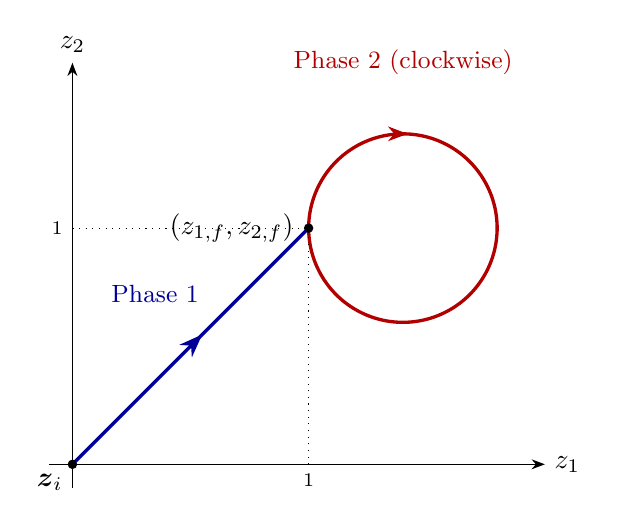
\begin{tikzpicture}[>=Stealth,scale=3.0]
  \draw[->] (-0.1,0) -- (2.0,0) node[right]{$z_1$};
  \draw[->] (0,-0.1) -- (0,1.7) node[above]{$z_2$};
  \draw[very thick,blue!60!black,
        decoration={markings,mark=at position 0.55 with {\arrow{Stealth}}},postaction={decorate}]
        (0,0) -- (1,1);
  \draw[very thick,red!70!black,smooth,samples=100,domain=0:360,variable=\t]
        plot({1+0.399*(1-cos(\t))},{1+0.399*sin(\t)});
  \draw[red!70!black,-{Stealth[length=2.5mm]}] (1.399,1.399) -- ++(0.02,-0.0);
  \fill (0,0) circle (0.02) node[below left]{$\z_i$};
  \fill (1,1) circle (0.02) node[left=2pt]{$(z_{1,f},z_{2,f})$};
  \node[blue!60!black,font=\small] at (0.35,0.72) {Phase 1};
  \node[red!70!black,font=\small] at (1.4,1.7) {Phase 2 (clockwise)};
  \draw[dotted] (1,0) -- (1,1); \draw[dotted] (0,1) -- (1,1);
  \node[below,font=\scriptsize] at (1,0) {1};
  \node[left,font=\scriptsize] at (0,1) {1};
\end{tikzpicture}
\caption{Trajectory in the $(z_1,z_2)$ plane for $\z_i=(0,0,0)$, $\z_f=(1,1,1)$ with $a=b$: a line (Phase~1) followed by a circle (Phase~2). The area enclosed by the circle, $\pi/(2\pi)=1/2$, is exactly the missing $\Delta z_3$.}
\end{figure}

\begin{figure}[H]
\centering
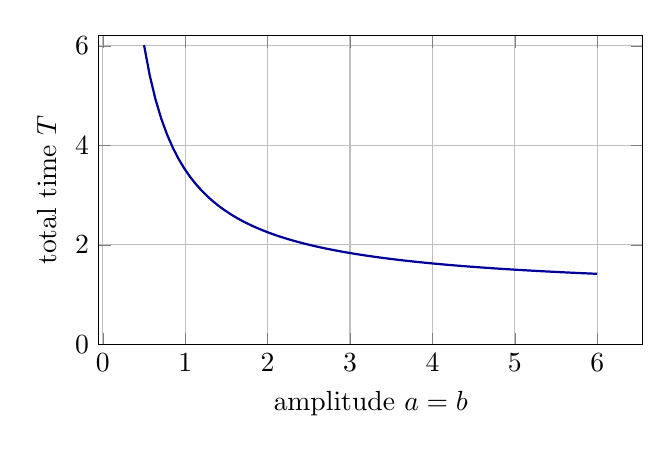
\begin{tikzpicture}
\begin{axis}[width=0.7\textwidth,height=5.5cm,xlabel={amplitude $a=b$},ylabel={total time $T$},
  grid=both,domain=0.5:6,samples=80,ymin=0,ymax=6.2]
  \addplot[thick,blue!60!black]{1+2.5066/x};
\end{axis}
\end{tikzpicture}
\caption{Trade-off for $\z_i=(0,0,0)\to\z_f=(1,1,1)$ with $a=b$: $T=1+\sqrt{2\pi}/a$. Larger input amplitude shortens Phase~2, which can never be shorter than zero, so $T\to T_1=1$.}
\end{figure}

%=====================================================================
\section{Front-Wheel-Drive Bicycle: Modelling, Flatness and Control}
\label{sec:bicycle}
%=====================================================================
\emph{(Midterm Class Test 2024/25, Problem~1)}

\begin{problem}{Problem statement}
Consider a bicycle robot of length $\ell$ with front-wheel drive. Define the configuration vector as $\q=(x_f,y_f,\theta,\phi)$, where $(x_f,y_f)$ are the Cartesian coordinates of the (contact point of the) front wheel, $\theta$ is the vehicle orientation, and $\phi$ is the steering angle of the front wheel.
\begin{enumerate}[label=(\alph*),nosep]
  \item Starting from the kinematic constraints acting on the system, derive a kinematic model of the vehicle with the front wheel driving and steering velocities as control inputs, and prove its controllability.
  \item Are $x_f,y_f$ flat outputs for this model? Motivate your answer and give an interpretation in terms of state/input reconstructability.
  \item Design a feedback controller for driving $x_f,y_f$ along a desired trajectory $x_f^*(t),y_f^*(t)$ and provide the corresponding block scheme. \emph{Hint: find an invertible mapping between the time derivative (of a suitable order) of the outputs and the dynamically extended control inputs.}
\end{enumerate}
\end{problem}


\subsection{Setting}

Consider a bicycle robot of length $\ell$ with front-wheel drive and configuration vector $\q=(x_f,y_f,\theta,\phi)^T$, where $(x_f,y_f)$ are the Cartesian coordinates of the contact point of the front wheel, $\theta$ is the vehicle orientation and $\phi$ is the steering angle of the front wheel.

\begin{figure}[H]
\centering
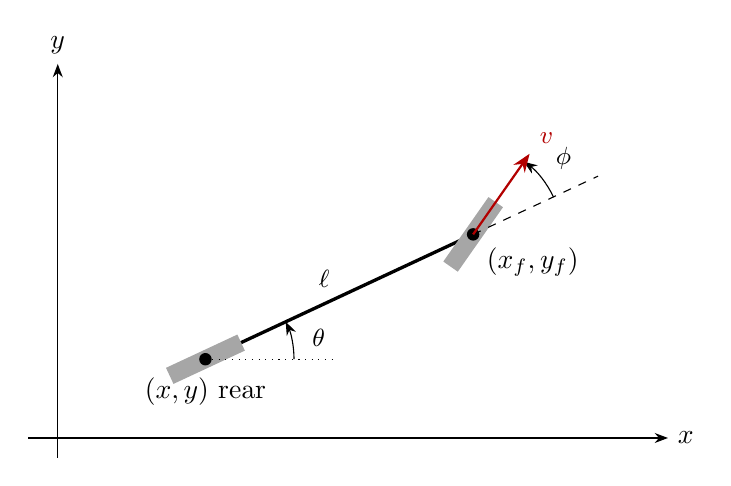
\begin{tikzpicture}[>=Stealth,scale=1.25]
  \draw[->] (-0.3,0) -- (6.2,0) node[right]{$x$};
  \draw[->] (0,-0.2) -- (0,3.8) node[above]{$y$};
  \coordinate (R) at (1.5,0.8);
  \coordinate (F) at ($(R)+(25:3)$);
  % body
  \draw[very thick] (R) -- (F);
  % rear wheel (orientation theta)
  \begin{scope}[shift={(R)},rotate=25]
    \fill[gray!70] (-0.4,-0.09) rectangle (0.4,0.09);
  \end{scope}
  % front wheel (orientation theta+phi)
  \begin{scope}[shift={(F)},rotate=55]
    \fill[gray!70] (-0.4,-0.09) rectangle (0.4,0.09);
  \end{scope}
  \draw[dashed] (F) -- ++(25:1.4);
  \draw[dotted] (R) -- ++(1.3,0);
  \draw[->] ($(R)+(0.9,0)$) arc[start angle=0,end angle=25,radius=0.9];
  \node[font=\small] at ($(R)+(1.15,0.22)$) {$\theta$};
  \draw[->] ($(F)+(25:0.9)$) arc[start angle=25,end angle=55,radius=0.9];
  \node[font=\small] at ($(F)+(40:1.2)$) {$\phi$};
  \fill (R) circle (1.8pt) node[below=3pt]{$(x,y)$ rear};
  \fill (F) circle (1.8pt) node[below right=2pt]{$(x_f,y_f)$};
  \node[font=\small,above left] at ($(R)!0.5!(F)$) {$\ell$};
  \draw[->,red!70!black,thick] (F) -- ++(55:1.0) node[above right,font=\small]{$v$};
\end{tikzpicture}
\caption{Front-wheel-drive bicycle. The front wheel has orientation $\theta+\phi$ and carries both drive ($v$) and steering ($\omega=\dot\phi$) inputs.}
\end{figure}

\subsection{(a) Kinematic model and controllability}

\paragraph{Constraints.} There is one pure-rolling condition per wheel (no lateral slip):
\begin{align}
  \dot x\sin\theta-\dot y\cos\theta&=0 &&\text{(rear wheel)}\\
  \dot x_f\sin(\theta+\phi)-\dot y_f\cos(\theta+\phi)&=0 &&\text{(front wheel)},
\end{align}
where $(x,y)$ are the coordinates of the rear wheel contact point, related to the front one by
\[
  x=x_f-\ell\cos\theta,\qquad y=y_f-\ell\sin\theta .
\]
Differentiating, $\dot x=\dot x_f+\ell\dot\theta\sin\theta$, $\dot y=\dot y_f-\ell\dot\theta\cos\theta$, and substituting into the rear constraint ($\sin^2\theta+\cos^2\theta=1$):
\[
  \dot x_f\sin\theta-\dot y_f\cos\theta+\ell\dot\theta=0 .
\]
In Pfaffian form, with $\q=(x_f,y_f,\theta,\phi)$,
\begin{equation}
  A^T(\q)\dot\q=
  \begin{pmatrix}
    \sin\theta & -\cos\theta & \ell & 0\\
    \sin(\theta+\phi) & -\cos(\theta+\phi) & 0 & 0
  \end{pmatrix}
  \begin{pmatrix}\dot x_f\\ \dot y_f\\ \dot\theta\\ \dot\phi\end{pmatrix}=0 .
\end{equation}
Here $n=4$ and $k=2$, so the null space is 2-dimensional.

\paragraph{Null-space basis and model.} A basis is
\[
  \g_1(\q)=\begin{pmatrix}\cos(\theta+\phi)\\ \sin(\theta+\phi)\\ \frac{\sin\phi}{\ell}\\0\end{pmatrix},\qquad
  \g_2(\q)=\begin{pmatrix}0\\0\\0\\1\end{pmatrix}.
\]
(Check: the second row of $A^T$ annihilates $\g_1$ because $\sin(\theta+\phi)\cos(\theta+\phi)-\cos(\theta+\phi)\sin(\theta+\phi)=0$; the first row gives $\sin\theta\cos(\theta+\phi)-\cos\theta\sin(\theta+\phi)+\sin\phi=-\sin\phi+\sin\phi=0$.) The kinematic model is
\begin{equation}
\boxed{\;
\begin{aligned}
  \dot x_f&=\cos(\theta+\phi)\,v\\
  \dot y_f&=\sin(\theta+\phi)\,v\\
  \dot\theta&=\frac{\sin\phi}{\ell}\,v\\
  \dot\phi&=\omega
\end{aligned}\;}
\label{eq:bike-km}
\end{equation}
where $v$ and $\omega$ are the driving and steering velocities, both generated at the front wheel.

\begin{intuition}
The front wheel can only move along its own heading $\theta+\phi$ (this is $v$). The rear wheel must follow, it cannot slip sideways, so the body turns at a rate $\frac{v\sin\phi}{\ell}$: it is the component of $v$ perpendicular to the body, divided by the lever arm $\ell$. If $\phi=0$ the vehicle goes straight; the larger the steering angle, the tighter the turn; at $\phi=\pm\pi/2$ the front wheel moves perpendicular to the body and the body pivots about the rear wheel. Steering is a separate, directly actuated velocity $\omega=\dot\phi$.
\end{intuition}

\paragraph{Controllability.} We compute the Lie brackets:
\[
  \g_3=[\g_1,\g_2]=\begin{pmatrix}\sin(\theta+\phi)\\-\cos(\theta+\phi)\\-\frac{\cos\phi}{\ell}\\0\end{pmatrix},\qquad
  \g_4=[\g_1,\g_3]=\begin{pmatrix}-\frac{\sin\theta}{\ell}\\ \frac{\cos\theta}{\ell}\\0\\0\end{pmatrix}.
\]
Then, reordering the columns,
\[
  \rank\begin{pmatrix}\g_1&\g_3&\g_4&\g_2\end{pmatrix}=
  \rank\begin{pmatrix}
    \cos(\theta+\phi)&\sin(\theta+\phi)&-\frac{\sin\theta}{\ell}&0\\
    \sin(\theta+\phi)&-\cos(\theta+\phi)&\frac{\cos\theta}{\ell}&0\\
    \frac{\sin\phi}{\ell}&-\frac{\cos\phi}{\ell}&0&0\\
    0&0&0&1
  \end{pmatrix}=4,
\]
because the determinant of the upper-left $3\times3$ block is $1/\ell^2\neq0$ (expand along the third column and use $\sin(\theta+\phi)\cos\theta-\cos(\theta+\phi)\sin\theta=\sin\phi$ and $\cos(\theta+\phi)\cos\theta+\sin(\theta+\phi)\sin\theta=\cos\phi$). The rank is 4 for every $\q$, so the kinematic model is \emph{controllable}.

\begin{intuition}
The bracket $\g_3$ is the ``wiggle the steering'' direction (drive a bit, steer, drive back, steer back), and $\g_4$ is the ``lateral'' direction perpendicular to the rear wheel. This is precisely the sideways motion that the constraint forbids directly but parallel parking obtains: the determinant $1/\ell^2$ never vanishes, so there is no configuration (not even $\phi=\pm\pi/2$) where this fails.
\end{intuition}

\subsection{(b) Are $x_f,y_f$ flat outputs?}

\paragraph{What can be reconstructed.} From the first two equations of \eqref{eq:bike-km},
\[
  \theta+\phi=\arctan\frac{\dot y_f}{\dot x_f},\qquad v=\pm\sqrt{\dot x_f^2+\dot y_f^2}
\]
(the sign of $v$ distinguishes forward from backward motion), and differentiating the first,
\begin{equation}
  \dot\theta+\dot\phi=\frac{\ddot y_f\dot x_f-\dot y_f\ddot x_f}{\dot x_f^2+\dot y_f^2}=:\kappa,\qquad\text{so}\quad \dot\theta=\kappa-\dot\phi .
\end{equation}

\paragraph{The obstruction.} From the third equation of \eqref{eq:bike-km}, $\sin\phi=\ell\dot\theta/v$, hence
\begin{equation}
  \phi=\arcsin\!\left[\frac{\ell}{v}\left(\frac{\ddot y_f\dot x_f-\dot y_f\ddot x_f}{\dot x_f^2+\dot y_f^2}-\dot\phi\right)\right],
  \qquad\text{equivalently}\qquad
  \dot\phi=\kappa-\frac{v}{\ell}\sin\phi .
  \label{eq:phi-ode}
\end{equation}
The right-hand side contains $\dot\phi$ itself: $\phi$ is the solution of a \emph{differential equation} driven by the outputs, not an algebraic function of them. Therefore $\phi$ (and consequently $\theta=\arctan(\dot y_f/\dot x_f)-\phi$) \emph{cannot be reconstructed algebraically} from $x_f,y_f$ and their derivatives:
\[
  \boxed{x_f,y_f\ \text{are \emph{not} flat outputs.}}
\]

\paragraph{Interpretation (state/input reconstructability).} Along a given front-wheel trajectory, $v$ and the heading $\theta+\phi$ of the front wheel are known, but the \emph{split} of this heading between body orientation $\theta$ and steering $\phi$ depends on the initial condition of \eqref{eq:phi-ode}. For the same front-wheel path there are infinitely many possible rear-wheel paths, one per initial condition.

\begin{figure}[H]
\centering
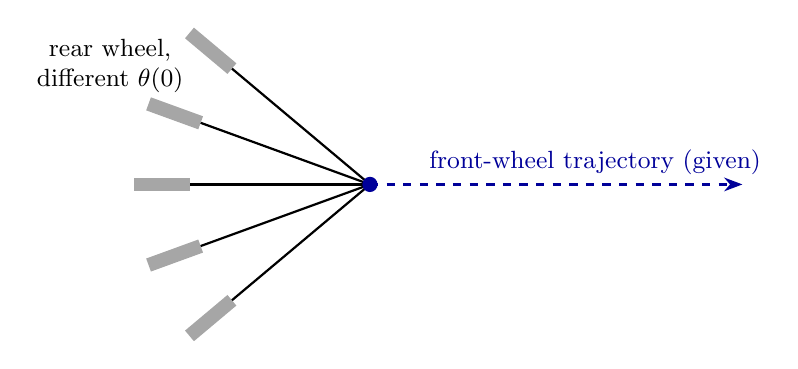
\begin{tikzpicture}[>=Stealth,scale=1.1]
  \coordinate (F) at (0,0);
  \foreach \a in {-40,-20,0,20,40}{
    \coordinate (R\a) at ($(F)-(\a:2.4)$);
    \draw[thick] (R\a) -- (F);
    \begin{scope}[shift={(R\a)},rotate=\a]
      \fill[gray!70] (-0.32,-0.08) rectangle (0.32,0.08);
    \end{scope}
  }
  \fill[blue!60!black] (F) circle (2.5pt);
  \draw[dashed,thick,blue!60!black,->] (F) -- (4.3,0);
  \node[above,font=\small,blue!60!black] at (2.6,0) {front-wheel trajectory (given)};
  \node[font=\small] at (-3.0,1.55) {rear wheel,};
  \node[font=\small] at (-3.0,1.2) {different $\theta(0)$};
\end{tikzpicture}
\caption{The same front-wheel path is compatible with infinitely many rear-wheel configurations, depending on the initial body orientation: this is why $(x_f,y_f)$ do not determine the state.}
\end{figure}

\begin{intuition}
It is a matter of what the front point alone can tell you. Suppose you only watch the front wheel moving along a straight line: is the car perfectly aligned behind it, or is the body at an angle, with the steering compensating? Both are consistent with the same front-wheel path. Which one is true is ``memory'' stored in $\phi$, and memory means integration, not algebra. Equation \eqref{eq:phi-ode} adds a further insight: for forward motion $v>0$ and $|\phi|<\pi/2$, the linearization $-\frac{v}{\ell}\cos\phi$ is negative, so the $\phi$-dynamics are \emph{stable} (the body aligns behind the front wheel, like a shopping cart caster); for backward motion the same ODE is \emph{unstable} (jackknifing).
\end{intuition}

\begin{remark}
A different choice of output \emph{does} work: for the bicycle with front-wheel drive, the Cartesian position of the \emph{rear} wheel is a flat output, because $\theta$ is recovered from the direction of its velocity (the rear wheel moves along the body axis), and $\phi$, $v$ then follow algebraically. The non-flatness above is specific to the front-wheel point.
\end{remark}

\subsection{(c) Tracking controller for $(x_f,y_f)$: dynamic feedback linearization}

\paragraph{Differentiate the outputs.} The first derivatives are $\dot x_f=\cos(\theta+\phi)v$, $\dot y_f=\sin(\theta+\phi)v$: only $v$ appears, so no decoupling is possible at this order (one input, two outputs). Differentiating again,
\begin{align*}
  \ddot x_f&=-\sin(\theta+\phi)(\dot\theta+\dot\phi)\,v+\cos(\theta+\phi)\,\dot v,\\
  \ddot y_f&=\ \ \cos(\theta+\phi)(\dot\theta+\dot\phi)\,v+\sin(\theta+\phi)\,\dot v .
\end{align*}

\paragraph{Dynamic extension.} Set $\dot v=a$ (the acceleration becomes the input, and $v$ becomes a state), and replace $\dot\theta=\frac{\sin\phi}{\ell}v$, $\dot\phi=\omega$:
\begin{equation}
  \begin{pmatrix}\ddot x_f\\ \ddot y_f\end{pmatrix}
  =\underbrace{\begin{pmatrix}-\sin(\theta+\phi)\frac{\sin\phi}{\ell}v^2\\[2pt] \ \ \cos(\theta+\phi)\frac{\sin\phi}{\ell}v^2\end{pmatrix}}_{\bb(\q,v)}
  +\underbrace{\begin{pmatrix}\cos(\theta+\phi)&-\sin(\theta+\phi)\,v\\ \sin(\theta+\phi)&\cos(\theta+\phi)\,v\end{pmatrix}}_{\Tm(\q,v)}
  \begin{pmatrix}a\\ \omega\end{pmatrix}.
\end{equation}
The decoupling matrix has $\det\Tm=v\neq0$: it is invertible whenever $v\ne0$. In this case
\[
  \Tm^{-1}(\q,v)=\frac1v\begin{pmatrix}v\cos(\theta+\phi)&v\sin(\theta+\phi)\\-\sin(\theta+\phi)&\cos(\theta+\phi)\end{pmatrix}.
\]

\paragraph{Linearizing law and tracking.} Let
\begin{equation}
  \begin{pmatrix}a\\ \omega\end{pmatrix}=\Tm^{-1}(\q,v)\left(\begin{pmatrix}u_1\\u_2\end{pmatrix}-\bb(\q,v)\right).
  \label{eq:fl}
\end{equation}
The system from $(u_1,u_2)$ to the outputs is then linear and decoupled,
\[
  \ddot x_f=u_1,\qquad \ddot y_f=u_2 .
\]
For a desired smooth trajectory $x_f^*(t),y_f^*(t)$ use the PD+feedforward law
\begin{align}
  u_1&=\ddot x_f^*+k_{p1}(x_f^*-x_f)+k_{d1}(\dot x_f^*-\dot x_f),\\
  u_2&=\ddot y_f^*+k_{p2}(y_f^*-y_f)+k_{d2}(\dot y_f^*-\dot y_f).
\end{align}
With $e_x=x_f^*-x_f$ the error obeys $\ddot e_x+k_{d1}\dot e_x+k_{p1}e_x=0$, whose characteristic polynomial $s^2+k_{d1}s+k_{p1}$ is Hurwitz iff $k_{p1},k_{d1}>0$; the same holds for $y$. Hence \emph{global exponential tracking} is obtained for any positive gains, as long as $v\neq0$.

\begin{figure}[H]
\centering
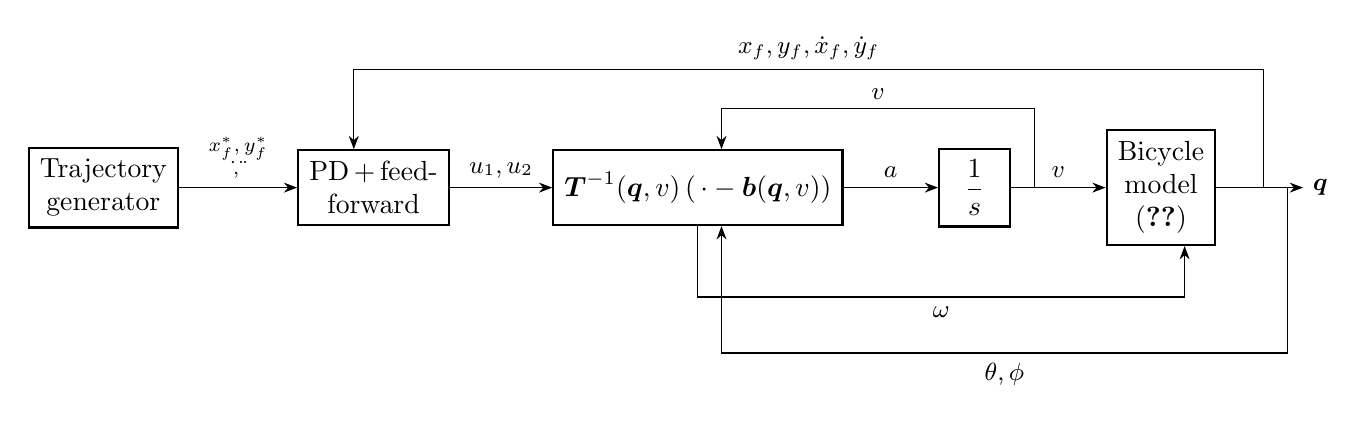
\begin{tikzpicture}[>=Stealth, node distance=1.2cm and 1.1cm,
  blk/.style={draw,thick,rectangle,minimum height=0.95cm,align=center,inner sep=4pt}]
  \node[blk] (gen) {Trajectory\\generator};
  \node[blk,right=1.5cm of gen] (pd) {PD\,+\,feed-\\forward};
  \node[blk,right=1.3cm of pd] (inv) {$\Tm^{-1}(\q,v)\,(\,\cdot-\bb(\q,v))$};
  \node[blk,right=1.2cm of inv,minimum width=0.9cm] (int) {$\dfrac1s$};
  \node[blk,right=1.2cm of int] (rob) {Bicycle\\model\\\eqref{eq:bike-km}};
  \draw[->] (gen) -- node[above,font=\scriptsize,align=center]{$x_f^*,y_f^*$\\$\dot{},\ddot{}$} (pd);
  \draw[->] (pd) -- node[above,font=\small]{$u_1,u_2$} (inv);
  \draw[->] (inv) -- node[above,font=\small]{$a$} (int);
  \draw[->] (int) -- node[above,font=\small]{$v$} (rob);
  % omega bypass
  \draw[->] (inv.south) -- ++(0,-0.9) -| node[pos=0.25,below,font=\small]{$\omega$} ([xshift=0.3cm]rob.south);
  % outputs
  \draw[->] (rob.east) -- ++(1.1,0) node[right,font=\small]{$\q$};
  % feedback of x_f,y_f,xdot,ydot to PD
  \draw[->] ($(rob.east)+(0.6,0)$) -- ++(0,1.5) -| node[pos=0.25,above,font=\small]{$x_f,y_f,\dot x_f,\dot y_f$} ([xshift=-0.25cm]pd.north);
  % feedback of q and v to inverse block
  \draw[->] ($(rob.east)+(0.9,0)$) -- ++(0,-2.1) -| node[pos=0.25,below,font=\small]{$\theta,\phi$} ([xshift=0.3cm]inv.south);
  \draw[->] ($(int.east)+(0.3,0)$) -- ++(0,1.0) -| node[pos=0.25,above,font=\small]{$v$} ([xshift=0.3cm]inv.north);
\end{tikzpicture}
\caption{Block scheme of the dynamic feedback linearizing controller for the front wheel. The integrator turns the acceleration input $a$ into the driving velocity $v$, so the controller is intrinsically dynamic (its state is $v$).}
\end{figure}

\paragraph{Practical remarks.}
\begin{itemize}[nosep]
  \item To compute $u_1,u_2$ one needs $x_f,y_f$ and their first derivatives. These can be obtained from the original measured states ($x,y,\theta$ or $x_f,y_f,\theta,\phi$), and in fact \emph{without numerical differentiation}, since $\dot x_f=\cos(\theta+\phi)v$ and $\dot y_f=\sin(\theta+\phi)v$ are known as soon as $\theta,\phi,v$ are.
  \item To compute $(a,\omega)$ through \eqref{eq:fl}, the angles $\theta,\phi$ and the extended state $v$ are needed.
  \item The driving velocity $v$ is obtained \emph{by integrating} $a$: the controller has an internal state, and must be initialized with $v(0)\neq0$.
\end{itemize}

\begin{intuition}
Why do we need to add an integrator? At the level of $\ddot x_f,\ddot y_f$ we have two outputs but, as long as $v$ is regarded as an input, a single actuator in the first derivatives. Delaying the appearance of $v$ by one step (treating $v$ as a state and $a$ as the input) gives two inputs $(a,\omega)$ that both show up in the second derivatives, and the matrix that multiplies them is invertible provided the vehicle is moving. The condition $v\neq0$ has a clear physical meaning: when the front wheel is at rest it cannot instantaneously accelerate \emph{sideways}: the steering input $\omega$ affects the front-wheel acceleration only through $v$ ($\omega\,v$ terms). Finally, the linearized dynamics have order $2+2=4$ whereas the extended system has order 5: the remaining state is the unobserved internal dynamics which is, again, the steering equation \eqref{eq:phi-ode}, stable for forward motion. This is consistent with part~(b).
\end{intuition}

%=====================================================================
\section{Summary}
\label{sec:summary}
%=====================================================================

\subsection{Comparison of the three problems}

\begin{table}[h]
\centering
\small
\renewcommand{\arraystretch}{1.3}
\begin{tabular}{p{2.5cm}p{3.7cm}p{4.1cm}p{4.0cm}}
\toprule
 & \textbf{Hopping robot} & \textbf{$(2,3)$ chained form} & \textbf{Front-wheel bicycle}\\
\midrule
State / inputs & $\q=(\phi,\ell,\theta)$; $u_1=\dot\phi$, $u_2=\dot\ell$ & $\z=(z_1,z_2,z_3)$; $v_1,v_2$ & $\q=(x_f,y_f,\theta,\phi)$; $v,\omega$\\
$n$, $k$ & $3,\ 1$ (angular momentum) & $3,\ 0$ (already a model) & $4,\ 2$ (rolling)\\
Controllable? & Yes: $[\g_1,\g_2]=(0,0,\tfrac{2m(d+\ell)}{J})^T$ & Yes: $[\g_1,\g_2]=(0,0,-1)^T$ & Yes: $\g_1,\g_2,[\g_1,\g_2],[\g_1,[\g_1,\g_2]]$ span, $\det=1/\ell^2$\\
Flatness & Flat for $d=0$; outputs $(\phi,\theta)$ & (Chain form is flat: $z_1,z_3$) & $(x_f,y_f)$ \emph{not} flat ($\phi$ via ODE)\\
Main tool & geometric model, polynomial interpolation of flat outputs & Two phases: integrate $z_1,z_2$; loop to fix $z_3$ & Dynamic extension $\dot v=a$, $\Tm^{-1}$\\
Result & Path planning; regulator $\theta\to0,\ \ell\to h$ & $T=T_1+2\pi/\omega$; $ab\pi/\omega^2=\Delta z_3$ & Exponential tracking of $x_f^*,y_f^*$ if $v\ne0$\\
Where it fails & $d+\ell=0$; $\dot\phi=0$; $\theta'$ must not change sign & $\omega\to0$ (slow) or large $a,b$ & $v=0$\\
\bottomrule
\end{tabular}
\caption{Side-by-side view of the three exercises.}
\end{table}

\subsection{Key points}

\begin{enumerate}
  \item \textbf{A velocity constraint is not a loss of reachability.} In all three systems the constraint is nonholonomic; brackets of the input vector fields (a leg cycle, a steering wiggle, an area swept in the $(z_1,z_2)$ plane) supply the ``missing'' directions, and the rank condition certifies it.
  \item \textbf{Choose the basis for interpretability.} The null space of the constraint admits many bases; take the one whose inputs are directly actuated ($\dot\phi,\dot\ell$ for the hopper; $v,\omega$ for the bicycle).
  \item \textbf{Flatness is a statement about algebra versus integration.} If a hidden variable is obtained by an algebraic formula (as $\ell$ from $\theta'/\phi'$), the output is flat and planning reduces to polynomial interpolation. If it requires solving an ODE (as $\phi$ from the front-wheel path), it is not flat: the same output curve hides infinitely many states.
  \item \textbf{Closed loops in the base variables generate net motion in the fiber.} The $\Delta\theta$ of the leg cycle and $\Delta z_3$ equal to the enclosed area are the same phenomenon, and give simple two-phase planners.
  \item \textbf{When the outputs are not flat, dynamic extension can still give exact tracking}, at the price of a singularity ($v=0$) and of leaving an internal dynamics (the steering angle) that must be stable.
\end{enumerate}

\end{document}